\chapter{Validation}

\section{Implémentation}
Deux outils principaux ont été utilisés pour avoir un logiciel le mieux écrit possible \ref{rails-tests}. Cette section les présente, premièrement, les tests unitaires, ensuite, les métriques.
%TODO faire intro

\subsection{Tests unitaires}
Les tests unitaires servent à vérifier que le code testé fonctionne correctement. L'implémentation des tests s'est déroulée en parallèle de la création de l'application. Durant la conception de Rsnap, deux principaux types de tests ont été réalisés, les tests sur les controlleurs et ceux au niveau de l'utilisateur. Mais avant tout, les outils utiliser pour ces test sont présenté.

\subsubsection{Outils pour les tests}
Pour réaliser ces tests, Travis-CI (\ref{travis}) est relié à Github pour que tout les tests soient exécuté à chaque commit. De plus, lors des "pull request" un message est affiché pour connaitre l'état de la branche. Le programmeur peut donc facilement savoir si l'acceptation de la branche introduira des bugs.

Une métrique générée par les tests est le couverture du code. Cette information est fournie par Coveralls\ref{biblio} qui est liée à Travis-CI pour l'aquisition des données. Cette métrique est utile pour connaître la fraction du code couvert par les tests. Elle ne donne par contre pas l'information du type de code testé, il faut donc faire attention que les tests couvrent les parties critiques.

Il est nécessaire de crée des données pour les modèles. Ceci s'effectue grâce au gem FactoryGirls \footnote{\url{https://github.com/thoughtbot/factory_girl_rails}} qui propose un langage dédié pour écrire rapidement des fabriques. Les fabriques vont a leur tour généré des données pour peuplé les modèles.

\subsubsection{Tests au niveau des controlleurs}
Une première série de tests est réalisée grâce à RSpec. Ces tests ont pour vocations de vérifier l'accès aux différentes routes : les droits des utilisateurs et le type de retour des contrôleurs.

Un exemple de test est visible sur dans le code source \ref{lst:rspec}. La partie \texttt{setup} utilise la fabrique spécifique pour créer une mission à chaque test. Deux tests sont ensuite réalisé qui vérifie que seul un utilisateur authentifié peut résourdre une mission.

\lstinputlisting[language=Ruby, caption={Test de l'accès au programme associé \`a une mission}, label=lst:rspec]{content/8-validation/validation/program_mission_initializations_controller_test.rb}

\subsubsection{Tests au niveau de l'utilisateur}
Une deuxième série de tests est réalisée grâce à Cucumber \ref{cucumber}. Cette deuxième série permet de tester l'application d'un point de vue utilisateur. Gerkin permet d'écrire les scénarii en langage naturel. Ce type de tests permet d'assurer que les fonctionnalités demandées par l'utilisateur fonctionne et donc toutes les ressources qui en dépende. Ces tests sont donc de haut niveaux car ce n'est que indirectement que des erreurs internes à l'application peuvent être trouvées via les interactions faites sur l'interface.

\lstinputlisting[language=Gherkin, caption={Tests de l'accès aux missions}, label=lst:cucumber-mission]{content/8-validation/validation/mission_access.feature}

\lstinputlisting[language=Ruby, linerange={1-15}, caption={Extrait de l'implémentation des tests de l'accès aux missions}, label=lst:cucumber-implementation-mission]{content/8-validation/validation/mission_steps.rb}
Le code source \ref{lst:cucumber-mission} montre différents scénarii décrivant l'accès aux missions. Le haut niveau de Gherkin est visible dans cet exemple. En effet, toute personne anglophone peut comprendre ce que teste les différents scénarii. 

L'extrait de code \ref{lst:cucumber-implementation-mission}, montre comment est implémenté les scénarii précédents. La facon dont est piloté un navigateur pour raliser les tests est aussi visible via par exemple les méthodes : \texttt{click\_on}, \texttt{current\_path}, \texttt{visit}\ldots

\subsection{Utilisation de metriques}%TODO ne suit pas la mm structure que dans connaissance nécessaire (metrique est dans test) 
Un autre style d'outil donne des informations sur le projet via le code source de celui-ci. Deux services ont principalement été utilisé.

\subsubsection{Gemnasium}
Gemnasium \ref{gemnasium} permet d'avoir un service de veille qui vérifie si les dépendance de l'application sont bien à jour et donc ne présente pas de risque de sécurité.

\subsubsection{rails\_best\_practice}
rails\_best\_practice \ref{rbp} fourni quand à lui une information plus complexe à traiter. En effet, il renseigne les endroits dans le code sources qui ne respecterait pas le "rails way". De plus, il fourni des exemple pour refactorer ceux-ci. Cet outil est donc utile principalement en début de projet quand les auteurs ne connaissent pas encore bien quelles sont les bonnes pratiques.

\section{Expériences}
Cette section aborde les expériences réalisées pour ce travail. Ceci commence par un après-midi chez kidscode en petit groupe avec des initiés, vient ensuite le printemps des sciences pendant lequel environ 80 élèves ont tester l'application. Enfin vient une analyse des expériences à travers des formulaires remplis par les élèves et les professeurs.
\subsection{kidscode}
\label{kidscode}
Dans le cadre de ce mémoire, plusieurs expériences ont été menées. La première s'est déroulée chez Kidscode. Cette organisation a été présentée dans la section \ref{init-kidscode}. C'est une petite initiative locale qui apprend la programmation à 10 enfants âgés de 10 à 14 ans.

\subsubsection{Contexte}
\label{context-kidscode}
Il est important de définir le contexte et le publique de l'expérience, car il peut avoir une influence considérable sur l'analyse de l'expérience.\\

Lors de cette expérience, le public était composé de 10 enfants de 10 à 14 ans ayant déjà fait une demi-année de programmation dans le cadre du projet Kidscode. Le niveau de ces enfants n'est donc pas à négliger. Ils sont habitués à exécuter un programme et maîtrisent les principaux concepts de la programmation.\\

\subsubsection{Buts}
Le but poursuivi dans cette expérience est de valider l'utilisabilité de la plateforme et également le niveau de difficulté des missions proposées. Un autre but était de se familiariser avec le public en petit groupe, en préparation de la seconde expérience.

Ce dernier point pourrait sembler être moins justifié dans le cadre d'un mémoire sur l'informatique, mais la manière d'aborder les enfants est tout aussi importante que la qualité de l'application. Pour limiter le plus possible les biais dus à un manque de pédagogie ou d'expérience dans la gestion d'un groupe d'enfant, il était important de pouvoir avoir cette première expérience.
\subsubsection{Déroulement}
L'expérience s'est déroulée pendant un peu plus d'une heure. Les enfants avaient dans les premières heures l'activité habituelle de kidscode et la dernière heure était dédiée à l'expérience. 

Comme le changement d'activité était clairement annoncé, le début de l'expérience fut marqué par beaucoup de pertes d'attention et de dissipations. Une fois le groupe repris en main, les jeunes ont directement montré beaucoup intérêt. Pour l'interface qu'ils découvraient qui semblait leur plaire, tout comme pour la compétition intergroupe qui s'est rapidement mis en place.\\

Comme expliqué dans la partie précédente \ref{context-kidscode}, le public avait déjà de bonnes notions de programmation par rapport au public visé par ce mémoire. Les premières missions sont donc passées très vite. Les seuls points de ralentissement étaient principalement des problèmes de lecture des consignes. 

À ce moment, les consignes étaient toutes uniquement écrites. Cela a posé un problème, car les jeunes ne prenaient pas le temps de les lire et donc ne savaient pas quoi faire. Ceci malgré la possibilité de retrouver les consignes dans les menus de l'application. Ce manque d'intérêt pour les consignes ne venait pas d'un problème de niveau de lecture, mais simplement d'une impatience face à l'expérience ce qui peut s'expliquer par le manque de rigueur dû à leur âge.\\

La compétition que les jeunes ont mise en place dès le début a eu un effet bénéfique pour leur évolution, car elle leur donnaient la motivation de réaliser les défis proposés. Ceci était fort marqué à chaque passage de missions. Chaque fois qu'un groupe finissait une mission, il était important pour eux de le signaler et cela leur donnait une satisfaction qui les poussait réaliser la mission suivante.\\ %d'ou le fait que plein de petites missions est approprier.

Dans les délais impartis, tous sont arrivés à la mission finale du chien et du chat \ref{chien-chat}, mais personne n'a réussi à la finir. Quand a sonné la fin de l'expérience, beaucoup nous ont demandé comment faire pour montrer ce qu'ils avaient réalisé à leur famille et comment faire pour continuer leurs réalisations.

\subsubsection{Analyse}
\label{analyse-kidscode}
L'expérience c'est dans l'ensemble très bien déroulée et les participants ont beaucoup apprécié.

Certaines améliorations ont été apportées à l'application due à cette expérience. Ces modifications seront discutées dans la suite de cette partie.

\paragraph{Changement dans les missions}
la mission \texttt{répète et répépète} a été retirée, car elle s'est avéré peu intéressante par rapport aux concepts introduits et peu accrocheuse pour les enfants. Cette mission avait pour but de faire découvrir les fonctions d'affichage de texte. Un personnage devait répéter ce que disait un autre. Pendant cette mission, beaucoup d'enfants se sont dispersés parce qu'ils s'embêtaient et que ce n'était pas assez concret. Cette mission a été remplacée par \texttt{Soyons courtois} décrite en section \ref{mission-courtois}. Cette nouvelle mission est beaucoup plus dynamique que la précédente, car elle permet à l'étudiant de se déplacer et utilise les capteurs de collisions introduits dans la mission précédente.

\paragraph{Ajout d'un bouton "reset"}
Lors de l'expérience, un groupe d'enfants a réussi suite à une série obscure d'opérations à corrompre l'environnement de la mission. Pour palier à ce genre de problème, un bouton "reset" a été rajouté dans l'interface de Snap! pour pouvoir réinitialiser la mission courante.

\paragraph{Ajout de vidéo d'introduction}
Comme observés dans cette expérience, les jeunes ont tendance à ne pas lire les textes explicatifs des missions. il en  résulte que les enfants ne savent pas quoi faire dans la mission et donc ne fond pas grand-chose de productif. Des vidéos d'introduction ont donc été rajoutées au début de chaque mission juste au dessus de l'explication de la mission. Cette vidéo explique le but de la mission et donne les instructions pour y arriver. Grâce à cela les étudiants regardent une fois la vidéo pour savoir ce qui leur est demandé. S'ils l'ont oublié, les consigne, un résumé écrit est toujours présent pour les rappeler.

% mission supprimer du a kidscode + bouton reset
% les viédo youtube
% nouveau bouton dans l'interface du a kidscode

\subsection{Scienceinfuse}
Cette expérience s'est déroulée dans le cadre de la semaine Scienceinfuse. Lors de cette dernière, des écoles du primaire et du secondaire viennent participer à des animations dans les universités. C'est lors de cette semaine Scienceinfuse que l'expérience s'est déroulée avec quatre groupes d'enfants de différent âge et horizon. Ces activités duraient au total une heure trente minutes avec les temps d'installation et de prise en charge. Lors de toutes ces activités, les élèves étaient en programmation par paire \ref{paire} et donc a deux devant un ordinateur. %TODO ref paire porgramming

\subsubsection{Contexte}
Le but de cette expérience dans le cadre de Scienceinfuse était de valider l'application sur un grand nombre d'enfants d'horizon et d'âge différent. Lors de cette expérience, 74 étudiants âgés de 11 ont 13 ans. Les enfants étaient répartis en 4 classes, deux de sixième primaire et deux de première humanité.

L'origine des jeunes est également variée. Il y a eu des classes de Chimay de Bousval et de Ottignies. Ceci est souhaité pour avoir un échantillon plus représentatif de la population.

\subsubsection{Buts}
Le but principal de cette expérience était de confronter l'application à son usage réel dans des classes d'étudiants. De pouvoir observer comment cela se déroule en réalité et ressortir une analyse des besoins spécifiques qui manqueraient à l'application.

Un autre but poursuivi était l'évaluation de l'âge idéal et du niveau de difficulté des missions pour des néophytes. En effet, lors de l'expérience précédente, le public était volontaire et avait déjà des connaissances en programmation. De par ce fait, le niveau des missions devait être réévalué sur le public visé.

Un dernier but était évidemment de récolter l'avis des personnes concernées, à savoir les étudiants, sur l'application. Observer leurs réactions et leurs intérêts ou non pour la solution proposée.

\subsubsection{Déroulement}
\paragraph{Déroulement général des activités}
Lors de la mise en place de l'activité, une petite démonstration de l'interface a été faite pour les familiariser à Snap!. 

Suite à cela les élèves ont été invités à créer un compte par groupe de deux (par ordinateur). La démonstration s'arrêtait à la première vidéo de la première mission.

Une fois la première vidéo passée, les élèves entament la première mission. Une crainte était que grâce au lecteur \texttt{youtube}, ils regardent d'autres vidéos, mais il n'en fût rien et leur curiosité était assez forte pour les garder dans l'application.\\

La première mission était celle de la voiture qui est décrite à la section \ref{mission-voiture}. Un des concepts difficiles abordés dans cette mission est la structuration mentale de leur script. C'est effectivement ce qui fût le plus difficile. La voiture revenait à son point de départ à chaque lancement du script. Mais finalement après quelque essaies-erreurs, ils ont tous réussi la mission.\\

Une fois la première mission finie, il était nécessaire de leur rappeler comment sauver et revenir à la liste des missions. Ensuite ils retrouvaient seuls comment faire. 

Une grande crainte des étudiants fut à chaque fois de savoir si leur mission avait bien été enregistrée sur le serveur.

À la fin, ils ont reçu un diplôme comportant surtout l'adresse web de l'application, dans le cas où ils souhaiteraient continuer leur programme chez eux.

\paragraph{École Sainte-Marie} 
La première classe à avoir testé la solution est celle de sixième primaire de l'école Sainte-Marie de Bousval. Le groupe était composé d'une petite vingtaine d'élèves.

L'activité s'est déroulée avec une petite contrariété informatique. En effet l'interpréteur JavaScript des machines mises à disposition était très lent. Ceci n'a pas compromis le déroulement de l'activité, mais fut à quelques moments une source de frustration pour certains élèves très enthousiastes.

À la fin du temps imparti, tous les élèves avaient atteint la dernière mission, chien et chat décrit en section \ref{chien-chat}. Ils n'ont généralement pas fini l'étape de déplacement du personnage, mais étaient bien avancés dans ce sens.

\paragraph{L'athénée royal Paule Delvaux}
Cette école est venue avec une classe de sixième primaire également. Pour cette école le problème de réactivité de l'interface a été corrigé.

Au niveau de la population et du niveau moyen des élèves, par rapport a l'école de Bousval, était légèrement plus faible et surtout les élève étaient moins autonome.\\

Pour l'activité les élèves sont arrivés un peu près à au même niveau que ceux de Bousval. Rien de spécial n'est à signaler.

L'enthousiasme des jeunes était également au rendez-vous et ils se sont bien amusés.

\paragraph{Collège saint Joseph}
Les deux dernières classes à participer à l'expérience étaient du collège saint Joseph de Chimay accompagner par leur professeur de mathématique. Ceci montre que ce public est intéressé par l'apprentissage de la logique de programmation.

Comme ces deux classes avaient un niveau de première humanité, leur prise en main a été plus simple, car les enfants étaient plus autonomes. L'expérience s'est déroulée comme pour les primaires. La première mission était la plus laborieuse, mais une fois passée tout allait très bien. Ces enfants étant plus grands, leur capacité d'apprentissage est également plus élevée. Ils ont donc été beaucoup plus rapides pour réaliser les missions. Ce qui leur a permis d'avancer beaucoup plus dans la dernière mission du chien et du chat. Certains groupes ont même eu un programme fonctionnel, il ne manquait que le score dont les étudiants n'ont pas eu le temps l'implémenter.\\

Une chose étonnant dans cette partie de l'expérience, c'est la différence de niveau au sein même de la classe. C'est une particularité qui était beaucoup moins marquée dans l'enseignement primaire. Dans ces groupes, même si la majorité se débrouillait très bien, certains groupes étaient complètement dépassés par les événements. Ils avaient besoin de plus de temps et d'aide pour y arriver. Ceci peut provenir de la différence de pédagogie entre le primaire où les enfants sont encore fort encadrés et l'enseignement d'humanité où les enfants doivent apprendre à se prendre en main.

Ces groupes moins fort ont très rapidement été démotivés et étaient difficiles à stimuler. Le manque d'expérience dans la gestion de groupes d'enfants a probablement, en autre, été un frein à leur motivation et à leur redynamisation.

Cette partie de l'expérience avec les classes d'humanités fut plus motivante, car les jeunes étaient plus dynamiques, mais surtout ils comprenaient mieux et plus rapidement les concepts enseignés.

\subsubsection{Analyse}
\label{analyse-scienceinfuse}
Cette expérience s’est très bien déroulée. Les objectifs ont été atteints. Le niveau des missions correspond à ce qui était souhaité. Les enfants ont très vite et bien pris en main l'interface de Snap!. Les modifications apportées par l'expérience précédente en section \ref{analyse-kidscode} ont été utiles. Il y avait en autre le bouton "reset" qui a été ajouté, a été utile et facile à utiliser. La mission \texttt{Soyons courtois}, voir section \ref{mission-courtois}, a été apprécié des enfants et remplis donc maintenant pleinement son rôle.\\ %TODO début fort condensé

Certaines nouvelles améliorations ont pu être trouvées. Parmi celles-ci, il y a l'ajout d'un message d'information sur la sauvegarde des projets. Une diminution du taux de rafraîchissement de la fenêtre. La mission hélicoptère qui introduit deux concepts : la boucle "répéter indéfiniment" et la condition "si". Il serait judicieux d'en faire deux missions séparées.

De manière générale, les enfants ont appris des concepts basiques de la programmation en une heure tout en s'amusant. À la fin de la séance, beaucoup d'enfants ne s'étaient pas rendu compte qu'autant de temps s'était passé.
% changement de la rate de rafraichissement
% les enfants ont appris sans s'en rendre compte
\subsection{analyse des résultats}
Dans cette partie seront discutés les résultats des expériences. Quelques statistiques sur les formulaires remplis par les enfants et les professeurs. Pour avoir les données complètes et les graphiques de ces données, ils sont en annexe en section \ref{annex-data-form}. S'y trouvent également tous les commentaires laissés par les élèves.

\paragraph{Niveau des enfants en informatique}
Comme dit plus haut, un formulaire a été compléter par les enfants à la fin de l'activité \ref{}. Une des questions portait sur leur connaissance de l'informatique et de la programmation avant et après l'activité. Les schémas \ref{fig:niveau-avant} montrent comment les enfants autoévaluaient leur compétence en informatique et en programmation avant de faire l'expérience. Les schémas \ref{fig:niveau-apres} montrent comment ils évaluent leur connaissance maintenant.
\begin{figure}[ht]
  \begin{center}
    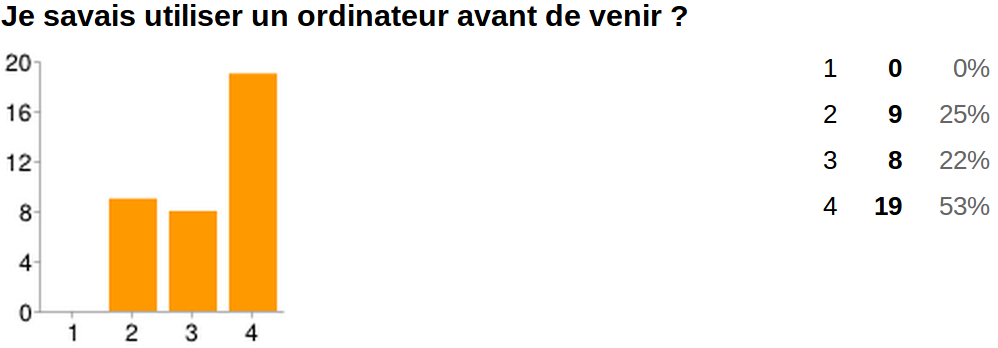
\includegraphics[scale=0.3]{content/8-validation/images/avant}
    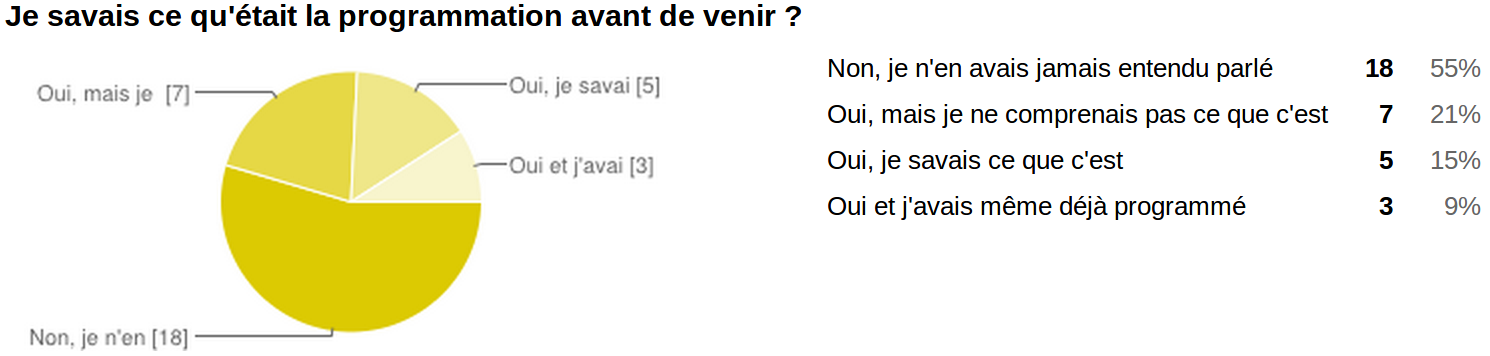
\includegraphics[scale=0.2]{content/8-validation/images/programmation}
    \caption{Auto estimation du niveau en informatique et en programmation des participants avant l'activité}
    \label{fig:niveau-avant}
  \end{center}
\end{figure}
\begin{figure}[ht]
  \begin{center}
    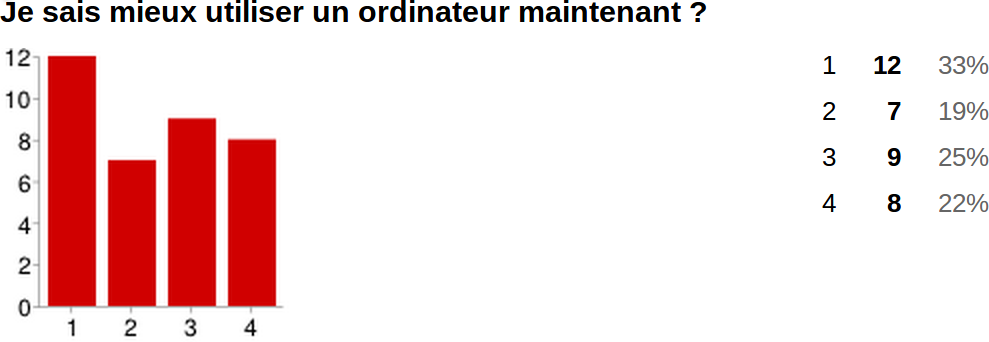
\includegraphics[scale=0.3]{content/8-validation/images/apres}
    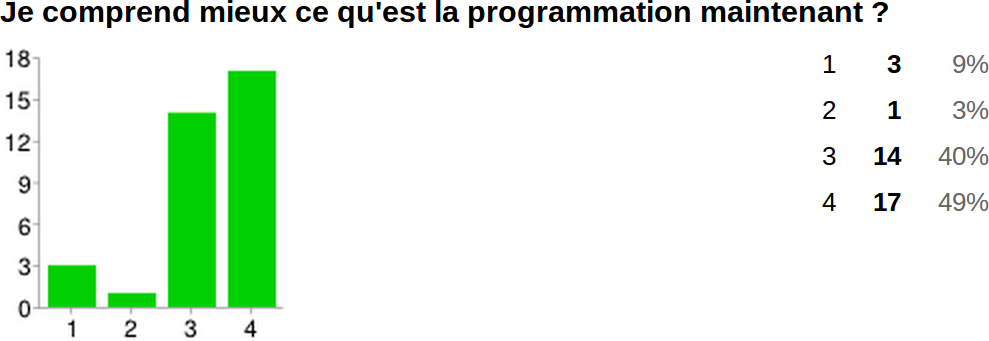
\includegraphics[scale=0.3]{content/8-validation/images/apres-programmation}
    \caption{Auto estimation du niveau en informatique et en programmation des participants après l'activité}
    \label{fig:niveau-apres}
  \end{center}
\end{figure}

\paragraph{Appréciation des missions}
\label{appreciation}
Au-delà de l'évaluation de leur niveau, ils ont également dû évaluer séparément chaque mission. Les graphiques représentant cette évaluation sont sur la figure \ref{fig:evaluation-mission}. On voit que les missions qui ont été le moins appréciées sont la troisième, soyons courtois, et la quatrième, chien et chat. La notation de la quatrième mission peut largement s'expliquer par la frustration qu'ils ont eue de ne pas avoir le temps de finir la mission. Pour la troisième, les retours indiquaient qu'ils avaient trouvé cette mission trop simple. Il faudrait repenser cette mission en y intégrant le déplacement du personnage par exemple.\\


\begin{figure}[ht]
  \begin{center}
    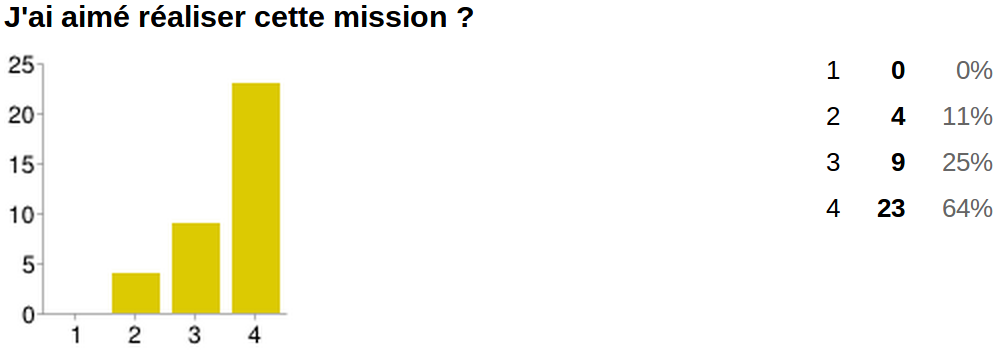
\includegraphics[scale=0.3]{content/8-validation/images/voiture}
    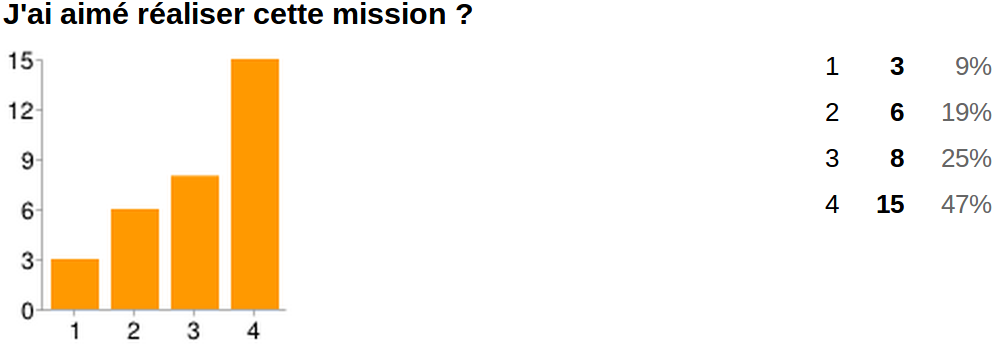
\includegraphics[scale=0.3]{content/8-validation/images/helico}
    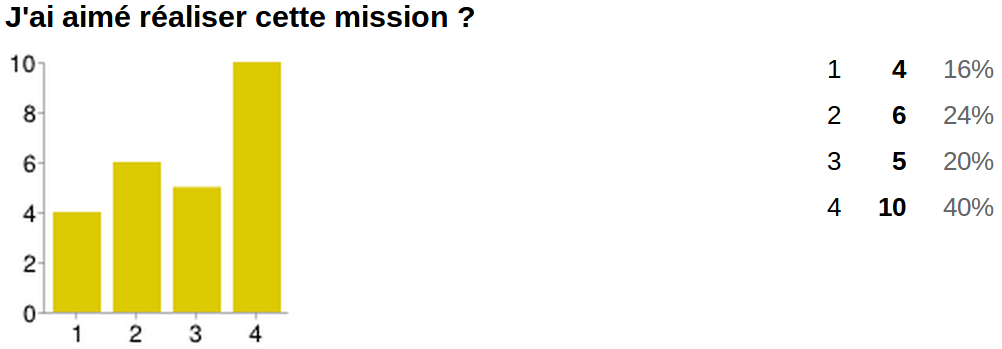
\includegraphics[scale=0.3]{content/8-validation/images/courtois}
    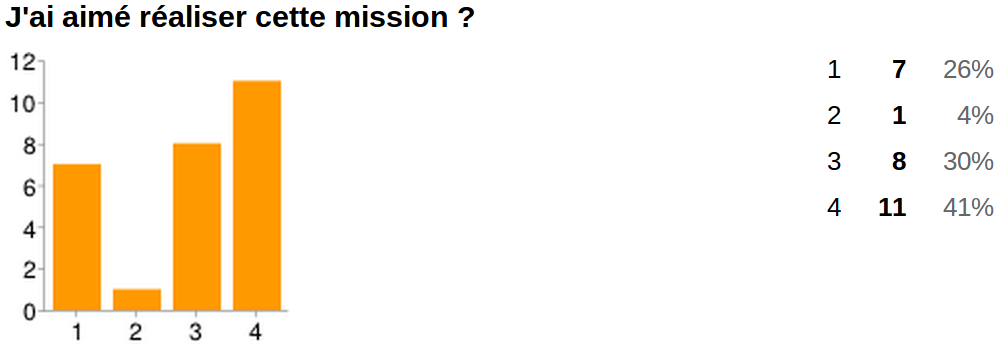
\includegraphics[scale=0.3]{content/8-validation/images/chien}
    \caption{Évaluation des missions par les enfants: En voiture \ref{mission-voiture}, hélicoptère \ref{mission-helicoptere}, soyons courtois \ref{mission-courtois}, tu ne m'attrapera jamais \ref{chien-chat}}
    \label{fig:evaluation-mission}
  \end{center}
\end{figure}

\paragraph{Appréciation des professeurs}
À propos des retours faits par les professeurs, ils sont en annexe \ref{result-prof}. Les retours étaient très positifs et les professeurs d'humanité étaient intéressés par l'application pour l'utiliser dans leurs cours.

\paragraph{Analyse des missions}
La première mission a été la plus laborieuse ce qui était prévu. Cependant, cette mission a le plus haut taux d'appréciation des enfants et donc en plus de remplir sa mission, elle est bien appréciée par ces derniers.\\

La seconde mission, celle de l'hélicoptère, a été appréciée, mais comme cité plus haut \ref{analyse-scienceinfuse}, elle pourrait être séparée en deux missions. Beaucoup d'étudiants ont eu besoin d'aide pour cumuler ces deux concepts en une fois.\\

La troisième mission, soyons courtois, est la moins appréciée, car trop facile. Une piste comme suggérée plus haut \ref{appreciation}, serait de rajouter l'implémentation des mouvements à cette mission.\\

La quatrième mission, chien et chat, a passionné les élèves, mais ils ont été frustrés par le manque de temps. Personne n'a réussi à la finir. Il faudrait peut-être plus guider les étudiants dans cette mission. Par exemple, tous les blocs étaient accessibles pour cette mission dans l'optique qu'ils puissent voir ce qui est possible de faire. A posteriori, ce n'est pas une bonne idée, car ils se perdent dans la masse de blocs disponibles.

\paragraph{Tranche d'âge}
Un objectif de ce travail est que les enfants puissent utiliser cette application de manière quasi autonome. Dans ce sens, les expériences ont montré que les enfants de début d'humanité sont plus aptes à travailler de manière autonome que les élèves de primaire.
Pour utiliser l'application avec des élèves de primaire, il faudra soit une plus grande maîtrise de la part du professeur soit plus d'encadrants.

% Les grands vont plus vite

% mission voiture cool pour la structuration
% débouché sur du concret

% différence d'age
% appréciation des missions



chiffre et analyse de notre formulaire prof et student.












<<<<<<< HEAD


=======
>>>>>>> rm image
